\documentclass[twoside]{book}

% Packages required by doxygen
\usepackage{calc}
\usepackage{doxygen}
\usepackage{graphicx}
\usepackage[utf8]{inputenc}
\usepackage{makeidx}
\usepackage{multicol}
\usepackage{multirow}
\PassOptionsToPackage{warn}{textcomp}
\usepackage{textcomp}
\usepackage[nointegrals]{wasysym}
\usepackage[table]{xcolor}

% Font selection
\usepackage[T1]{fontenc}
\usepackage{mathptmx}
\usepackage[scaled=.90]{helvet}
\usepackage{courier}
\usepackage{amssymb}
\usepackage{sectsty}
\renewcommand{\familydefault}{\sfdefault}
\allsectionsfont{%
  \fontseries{bc}\selectfont%
  \color{darkgray}%
}
\renewcommand{\DoxyLabelFont}{%
  \fontseries{bc}\selectfont%
  \color{darkgray}%
}
\newcommand{\+}{\discretionary{\mbox{\scriptsize$\hookleftarrow$}}{}{}}

% Page & text layout
\usepackage{geometry}
\geometry{%
  a4paper,%
  top=2.5cm,%
  bottom=2.5cm,%
  left=2.5cm,%
  right=2.5cm%
}
\tolerance=750
\hfuzz=15pt
\hbadness=750
\setlength{\emergencystretch}{15pt}
\setlength{\parindent}{0cm}
\setlength{\parskip}{0.2cm}
\makeatletter
\renewcommand{\paragraph}{%
  \@startsection{paragraph}{4}{0ex}{-1.0ex}{1.0ex}{%
    \normalfont\normalsize\bfseries\SS@parafont%
  }%
}
\renewcommand{\subparagraph}{%
  \@startsection{subparagraph}{5}{0ex}{-1.0ex}{1.0ex}{%
    \normalfont\normalsize\bfseries\SS@subparafont%
  }%
}
\makeatother

% Headers & footers
\usepackage{fancyhdr}
\pagestyle{fancyplain}
\fancyhead[LE]{\fancyplain{}{\bfseries\thepage}}
\fancyhead[CE]{\fancyplain{}{}}
\fancyhead[RE]{\fancyplain{}{\bfseries\leftmark}}
\fancyhead[LO]{\fancyplain{}{\bfseries\rightmark}}
\fancyhead[CO]{\fancyplain{}{}}
\fancyhead[RO]{\fancyplain{}{\bfseries\thepage}}
\fancyfoot[LE]{\fancyplain{}{}}
\fancyfoot[CE]{\fancyplain{}{}}
\fancyfoot[RE]{\fancyplain{}{\bfseries\scriptsize Generated on Fri Mar 7 2014 00\+:15\+:20 for My Project by Doxygen }}
\fancyfoot[LO]{\fancyplain{}{\bfseries\scriptsize Generated on Fri Mar 7 2014 00\+:15\+:20 for My Project by Doxygen }}
\fancyfoot[CO]{\fancyplain{}{}}
\fancyfoot[RO]{\fancyplain{}{}}
\renewcommand{\footrulewidth}{0.4pt}
\renewcommand{\chaptermark}[1]{%
  \markboth{#1}{}%
}
\renewcommand{\sectionmark}[1]{%
  \markright{\thesection\ #1}%
}

% Indices & bibliography
\usepackage{natbib}
\usepackage[titles]{tocloft}
\setcounter{tocdepth}{3}
\setcounter{secnumdepth}{5}
\makeindex

% Hyperlinks (required, but should be loaded last)
\usepackage{ifpdf}
\ifpdf
  \usepackage[pdftex,pagebackref=true]{hyperref}
\else
  \usepackage[ps2pdf,pagebackref=true]{hyperref}
\fi
\hypersetup{%
  colorlinks=true,%
  linkcolor=blue,%
  citecolor=blue,%
  unicode%
}

% Custom commands
\newcommand{\clearemptydoublepage}{%
  \newpage{\pagestyle{empty}\cleardoublepage}%
}


%===== C O N T E N T S =====

\begin{document}

% Titlepage & ToC
\hypersetup{pageanchor=false,
             bookmarks=true,
             bookmarksnumbered=true,
             pdfencoding=unicode
            }
\pagenumbering{roman}
\begin{titlepage}
\vspace*{7cm}
\begin{center}%
{\Large My Project }\\
\vspace*{1cm}
{\large Generated by Doxygen 1.8.6}\\
\vspace*{0.5cm}
{\small Fri Mar 7 2014 00:15:20}\\
\end{center}
\end{titlepage}
\clearemptydoublepage
\tableofcontents
\clearemptydoublepage
\pagenumbering{arabic}
\hypersetup{pageanchor=true}

%--- Begin generated contents ---
\chapter{Hierarchical Index}
\section{Class Hierarchy}
This inheritance list is sorted roughly, but not completely, alphabetically\+:\begin{DoxyCompactList}
\item Q\+G\+L\+Widget\begin{DoxyCompactList}
\item \contentsline{section}{glrenderer}{\pageref{classglrenderer}}{}
\end{DoxyCompactList}
\item Q\+Main\+Window\begin{DoxyCompactList}
\item \contentsline{section}{Main\+Window}{\pageref{class_main_window}}{}
\end{DoxyCompactList}
\item Sound\+Stream\begin{DoxyCompactList}
\item \contentsline{section}{sfe\+:\+:Sequential\+Sound\+Streamer}{\pageref{classsfe_1_1_sequential_sound_streamer}}{}
\end{DoxyCompactList}
\item \contentsline{section}{Turing}{\pageref{class_turing}}{}
\item \contentsline{section}{Ui\+\_\+\+Main\+Window}{\pageref{class_ui___main_window}}{}
\begin{DoxyCompactList}
\item \contentsline{section}{Ui\+:\+:Main\+Window}{\pageref{class_ui_1_1_main_window}}{}
\end{DoxyCompactList}
\end{DoxyCompactList}

\chapter{Class Index}
\section{Class List}
Here are the classes, structs, unions and interfaces with brief descriptions\+:\begin{DoxyCompactList}
\item\contentsline{section}{\hyperlink{classglrenderer}{glrenderer} }{\pageref{classglrenderer}}{}
\item\contentsline{section}{\hyperlink{class_main_window}{Main\+Window} }{\pageref{class_main_window}}{}
\item\contentsline{section}{\hyperlink{class_ui_1_1_main_window}{Ui\+::\+Main\+Window} }{\pageref{class_ui_1_1_main_window}}{}
\item\contentsline{section}{\hyperlink{classsfe_1_1_sequential_sound_streamer}{sfe\+::\+Sequential\+Sound\+Streamer} }{\pageref{classsfe_1_1_sequential_sound_streamer}}{}
\item\contentsline{section}{\hyperlink{class_turing}{Turing} }{\pageref{class_turing}}{}
\item\contentsline{section}{\hyperlink{class_ui___main_window}{Ui\+\_\+\+Main\+Window} }{\pageref{class_ui___main_window}}{}
\end{DoxyCompactList}

\chapter{Class Documentation}
\hypertarget{classglrenderer}{\section{glrenderer Class Reference}
\label{classglrenderer}\index{glrenderer@{glrenderer}}
}
Inheritance diagram for glrenderer\+:\begin{figure}[H]
\begin{center}
\leavevmode
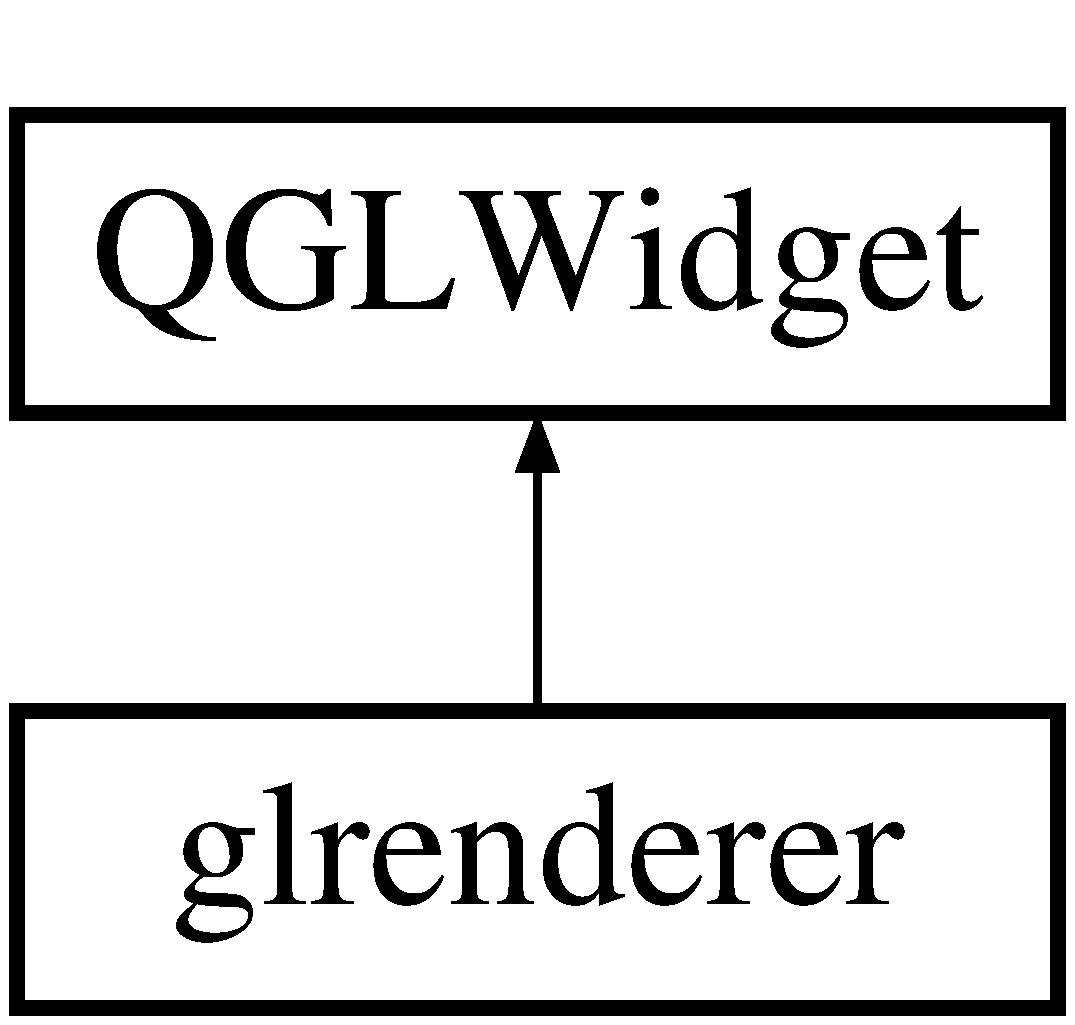
\includegraphics[height=2.000000cm]{classglrenderer}
\end{center}
\end{figure}
\subsection*{Public Member Functions}
\begin{DoxyCompactItemize}
\item 
\hypertarget{classglrenderer_acb574b369f4dd78d048ef4703c017c1a}{void \hyperlink{classglrenderer_acb574b369f4dd78d048ef4703c017c1a}{load\+Shaders} ()}\label{classglrenderer_acb574b369f4dd78d048ef4703c017c1a}

\begin{DoxyCompactList}\small\item\em load\+Shaders loads all available shaders \end{DoxyCompactList}\item 
void \hyperlink{classglrenderer_aef045836076110d931a2a372a7cfb3ff}{load\+Sound\+File} (const std\+::string \&filename)
\begin{DoxyCompactList}\small\item\em load\+Sound\+File loads a sound file at a given filename \end{DoxyCompactList}\end{DoxyCompactItemize}
\subsection*{Protected Member Functions}
\begin{DoxyCompactItemize}
\item 
\hypertarget{classglrenderer_ac168f504d3dc873dd032c996c962ad90}{void \hyperlink{classglrenderer_ac168f504d3dc873dd032c996c962ad90}{initialize\+G\+L} ()}\label{classglrenderer_ac168f504d3dc873dd032c996c962ad90}

\begin{DoxyCompactList}\small\item\em initialize\+G\+L Calls several functions to setup the initial G\+L state. \end{DoxyCompactList}\item 
\hypertarget{classglrenderer_a79e6616b1c2c34801742aaf69fc6e5df}{void {\bfseries paint\+G\+L} ()}\label{classglrenderer_a79e6616b1c2c34801742aaf69fc6e5df}

\item 
\hypertarget{classglrenderer_aee012c84c43499364df0c97a160169cf}{void {\bfseries update\+G\+L} ()}\label{classglrenderer_aee012c84c43499364df0c97a160169cf}

\item 
void \hyperlink{classglrenderer_a1743b7d54ffad4131e877486a99a568c}{resize\+G\+L} (int width, int height)
\begin{DoxyCompactList}\small\item\em resize\+G\+L callback for reshaping the window \end{DoxyCompactList}\end{DoxyCompactItemize}
\subsection*{Private Member Functions}
\begin{DoxyCompactItemize}
\item 
void \hyperlink{classglrenderer_ab90e6a3eca112f7048b36940c6f9f7ab}{print\+Shader\+Log} (G\+Luint obj)
\begin{DoxyCompactList}\small\item\em print\+Shader\+Log prints out any compilation errors, etc. generated from the creation of this G\+L object \end{DoxyCompactList}\item 
void \hyperlink{classglrenderer_ae809cfd8ed84e1596fc2b6295faee1e6}{print\+Program\+Log} (G\+Luint obj)
\begin{DoxyCompactList}\small\item\em prints out any compilation errors, etc. generated from the creation of this G\+L object \end{DoxyCompactList}\item 
G\+Lint \hyperlink{classglrenderer_ac2520771e2459563dcbfc98fb48431c3}{init\+Shader} (std\+::string \&vert\+File\+Name, std\+::string \&frag\+File\+Name)
\begin{DoxyCompactList}\small\item\em init\+Shader generates a shader program object from the given vertex and fragment source files \end{DoxyCompactList}\item 
\hypertarget{classglrenderer_a89899cb659769f33bd8e2610527a421e}{void \hyperlink{classglrenderer_a89899cb659769f33bd8e2610527a421e}{init\+Shaders} ()}\label{classglrenderer_a89899cb659769f33bd8e2610527a421e}

\begin{DoxyCompactList}\small\item\em init\+Shaders generates a bunch of shaders. \end{DoxyCompactList}\item 
\hypertarget{classglrenderer_a55618adb9e0917c835e52a3d256ef1d3}{void \hyperlink{classglrenderer_a55618adb9e0917c835e52a3d256ef1d3}{init\+Buffers} ()}\label{classglrenderer_a55618adb9e0917c835e52a3d256ef1d3}

\begin{DoxyCompactList}\small\item\em init\+Buffers initializes frame buffer objects for render to texture procedures \end{DoxyCompactList}\item 
void \hyperlink{classglrenderer_ad59e653833eaab9f9eb1e60ef3cec332}{render\+Grid} (float minx, float maxx, float miny, float maxy, float dx, float dy)
\begin{DoxyCompactList}\small\item\em render\+Grid Renders a grid of points to be passed to a shader. The positions of the points are somewhat arbitrary, since they will be sent to the shader anyways. \end{DoxyCompactList}\item 
\hypertarget{classglrenderer_a7e1a9ca2d682ef93705dd85d27dec830}{void \hyperlink{classglrenderer_a7e1a9ca2d682ef93705dd85d27dec830}{render} ()}\label{classglrenderer_a7e1a9ca2d682ef93705dd85d27dec830}

\begin{DoxyCompactList}\small\item\em render called during the \char`\"{}paint\+G\+L\char`\"{} callback. Runs approximately 60\+F\+P\+S, although this number is not static and cannot be assumed! \end{DoxyCompactList}\item 
\hypertarget{classglrenderer_a7751070a6f58b09f9b027e59d7533011}{void {\bfseries init\+Sound\+Stream} ()}\label{classglrenderer_a7751070a6f58b09f9b027e59d7533011}

\item 
\hypertarget{classglrenderer_a27bd7bcc2c4defe5152816e8e8ac690c}{void {\bfseries render\+F\+F\+T} (double $\ast$data\+Abs)}\label{classglrenderer_a27bd7bcc2c4defe5152816e8e8ac690c}

\item 
\hypertarget{classglrenderer_a80b4fe511f5c6cc6a09c7daf4f3f3d62}{void {\bfseries render\+To\+Texture} ()}\label{classglrenderer_a80b4fe511f5c6cc6a09c7daf4f3f3d62}

\item 
\hypertarget{classglrenderer_ad79d4e42fb594df49bde8ea5765151fc}{glm\+::vec3 {\bfseries H\+S\+Vto\+R\+G\+B} (float h, float s, float v)}\label{classglrenderer_ad79d4e42fb594df49bde8ea5765151fc}

\end{DoxyCompactItemize}
\subsection*{Private Attributes}
\begin{DoxyCompactItemize}
\item 
\hypertarget{classglrenderer_a6d797cf041a7b0e41d2fb7143e5cdd50}{glm\+::vec2 {\bfseries dim\+\_\+}}\label{classglrenderer_a6d797cf041a7b0e41d2fb7143e5cdd50}

\item 
\hypertarget{classglrenderer_acfd79b958ddd8151a6f309a699ee7993}{std\+::vector$<$ G\+Luint $>$ \hyperlink{classglrenderer_acfd79b958ddd8151a6f309a699ee7993}{shaders}}\label{classglrenderer_acfd79b958ddd8151a6f309a699ee7993}

\begin{DoxyCompactList}\small\item\em shaders a list of all G\+Luints that link to a shader \end{DoxyCompactList}\item 
\hypertarget{classglrenderer_ad66b91cdaa22164b04bed33c5cb871e5}{float \hyperlink{classglrenderer_ad66b91cdaa22164b04bed33c5cb871e5}{t\+\_\+}}\label{classglrenderer_ad66b91cdaa22164b04bed33c5cb871e5}

\begin{DoxyCompactList}\small\item\em t current time \end{DoxyCompactList}\item 
\hypertarget{classglrenderer_ac4458e650ddb3f8a2ed453894f90c678}{float \hyperlink{classglrenderer_ac4458e650ddb3f8a2ed453894f90c678}{last\+\_\+t\+\_\+}}\label{classglrenderer_ac4458e650ddb3f8a2ed453894f90c678}

\begin{DoxyCompactList}\small\item\em last\+\_\+t time of last frame \end{DoxyCompactList}\item 
\hypertarget{classglrenderer_a817bd1af09fff95e86e34ccc888f5424}{\hyperlink{classsfe_1_1_sequential_sound_streamer}{sfe\+::\+Sequential\+Sound\+Streamer} $\ast$ \hyperlink{classglrenderer_a817bd1af09fff95e86e34ccc888f5424}{soundstream\+\_\+}}\label{classglrenderer_a817bd1af09fff95e86e34ccc888f5424}

\begin{DoxyCompactList}\small\item\em soundstream used to stream sound data \end{DoxyCompactList}\item 
\hypertarget{classglrenderer_a91c7277b1eaef67da6e862123ddbfa38}{float \hyperlink{classglrenderer_a91c7277b1eaef67da6e862123ddbfa38}{sound\+\_\+t\+\_\+}}\label{classglrenderer_a91c7277b1eaef67da6e862123ddbfa38}

\begin{DoxyCompactList}\small\item\em sound\+\_\+t time of current sound \end{DoxyCompactList}\item 
\hypertarget{classglrenderer_a9290e152323d6ea26964685e5aa8b547}{G\+Luint \hyperlink{classglrenderer_a9290e152323d6ea26964685e5aa8b547}{fbo}}\label{classglrenderer_a9290e152323d6ea26964685e5aa8b547}

\begin{DoxyCompactList}\small\item\em fbo pixel buffer object for the output pixels \end{DoxyCompactList}\item 
\hypertarget{classglrenderer_a5f72e06bbeea3d339200ecc30be840d7}{G\+Luint $\ast$ \hyperlink{classglrenderer_a5f72e06bbeea3d339200ecc30be840d7}{vbo}}\label{classglrenderer_a5f72e06bbeea3d339200ecc30be840d7}

\begin{DoxyCompactList}\small\item\em vbo pixel buffer object for calculating variance \end{DoxyCompactList}\item 
\hypertarget{classglrenderer_a7df05aa3b22a05dc12e13d0d624bd0c0}{G\+Luint {\bfseries dbo}}\label{classglrenderer_a7df05aa3b22a05dc12e13d0d624bd0c0}

\item 
\hypertarget{classglrenderer_a122c79aaf9596256554145d36b134c0f}{G\+Luint {\bfseries pixels\+\_\+} \mbox{[}2\mbox{]}}\label{classglrenderer_a122c79aaf9596256554145d36b134c0f}

\item 
\hypertarget{classglrenderer_aec06d37529a85996e6a07f92782870c1}{G\+Luint {\bfseries sound\+Tex}}\label{classglrenderer_aec06d37529a85996e6a07f92782870c1}

\item 
\hypertarget{classglrenderer_acfa2e1407c1dcb33c143f946b86c7eb5}{G\+Luint {\bfseries sound\+Tex\+Loc\+\_\+}}\label{classglrenderer_acfa2e1407c1dcb33c143f946b86c7eb5}

\item 
\hypertarget{classglrenderer_ad57c1067763fa41daf76bb9df001c746}{G\+Luint {\bfseries pixel\+Tex\+Loc\+\_\+}}\label{classglrenderer_ad57c1067763fa41daf76bb9df001c746}

\item 
\hypertarget{classglrenderer_adae4055c80604f2c8b157764edb1c6b9}{size\+\_\+t {\bfseries buffersize\+\_\+}}\label{classglrenderer_adae4055c80604f2c8b157764edb1c6b9}

\item 
\hypertarget{classglrenderer_acfb55ec6086c39e4e248f843f935dc65}{Q\+Timer {\bfseries timer\+\_\+}}\label{classglrenderer_acfb55ec6086c39e4e248f843f935dc65}

\item 
\hypertarget{classglrenderer_a9d34cb31d4727ae4c117c7201c1e2591}{Q\+Elapsed\+Timer {\bfseries etimer\+\_\+}}\label{classglrenderer_a9d34cb31d4727ae4c117c7201c1e2591}

\item 
\hypertarget{classglrenderer_ab5e4d8b9d4611bbba87a9f813eda8c74}{int {\bfseries pingpong}}\label{classglrenderer_ab5e4d8b9d4611bbba87a9f813eda8c74}

\end{DoxyCompactItemize}


\subsection{Member Function Documentation}
\hypertarget{classglrenderer_ac2520771e2459563dcbfc98fb48431c3}{\index{glrenderer@{glrenderer}!init\+Shader@{init\+Shader}}
\index{init\+Shader@{init\+Shader}!glrenderer@{glrenderer}}
\subsubsection[{init\+Shader}]{\setlength{\rightskip}{0pt plus 5cm}G\+Lint glrenderer\+::init\+Shader (
\begin{DoxyParamCaption}
\item[{std\+::string \&}]{vert\+File\+Name, }
\item[{std\+::string \&}]{frag\+File\+Name}
\end{DoxyParamCaption}
)\hspace{0.3cm}{\ttfamily [private]}}}\label{classglrenderer_ac2520771e2459563dcbfc98fb48431c3}


init\+Shader generates a shader program object from the given vertex and fragment source files 


\begin{DoxyParams}{Parameters}
{\em vert\+File\+Name} & vertex shader source filename \\
\hline
{\em frag\+File\+Name} & fragment shader source filename \\
\hline
\end{DoxyParams}
\begin{DoxyReturn}{Returns}
shader program object 
\end{DoxyReturn}
\hypertarget{classglrenderer_aef045836076110d931a2a372a7cfb3ff}{\index{glrenderer@{glrenderer}!load\+Sound\+File@{load\+Sound\+File}}
\index{load\+Sound\+File@{load\+Sound\+File}!glrenderer@{glrenderer}}
\subsubsection[{load\+Sound\+File}]{\setlength{\rightskip}{0pt plus 5cm}void glrenderer\+::load\+Sound\+File (
\begin{DoxyParamCaption}
\item[{const std\+::string \&}]{filename}
\end{DoxyParamCaption}
)}}\label{classglrenderer_aef045836076110d931a2a372a7cfb3ff}


load\+Sound\+File loads a sound file at a given filename 


\begin{DoxyParams}{Parameters}
{\em filename} & the location of the file to be played \\
\hline
\end{DoxyParams}
\hypertarget{classglrenderer_ae809cfd8ed84e1596fc2b6295faee1e6}{\index{glrenderer@{glrenderer}!print\+Program\+Log@{print\+Program\+Log}}
\index{print\+Program\+Log@{print\+Program\+Log}!glrenderer@{glrenderer}}
\subsubsection[{print\+Program\+Log}]{\setlength{\rightskip}{0pt plus 5cm}void glrenderer\+::print\+Program\+Log (
\begin{DoxyParamCaption}
\item[{G\+Luint}]{obj}
\end{DoxyParamCaption}
)\hspace{0.3cm}{\ttfamily [private]}}}\label{classglrenderer_ae809cfd8ed84e1596fc2b6295faee1e6}


prints out any compilation errors, etc. generated from the creation of this G\+L object 


\begin{DoxyParams}{Parameters}
{\em obj} & shader object I\+D \\
\hline
\end{DoxyParams}
\hypertarget{classglrenderer_ab90e6a3eca112f7048b36940c6f9f7ab}{\index{glrenderer@{glrenderer}!print\+Shader\+Log@{print\+Shader\+Log}}
\index{print\+Shader\+Log@{print\+Shader\+Log}!glrenderer@{glrenderer}}
\subsubsection[{print\+Shader\+Log}]{\setlength{\rightskip}{0pt plus 5cm}void glrenderer\+::print\+Shader\+Log (
\begin{DoxyParamCaption}
\item[{G\+Luint}]{obj}
\end{DoxyParamCaption}
)\hspace{0.3cm}{\ttfamily [private]}}}\label{classglrenderer_ab90e6a3eca112f7048b36940c6f9f7ab}


print\+Shader\+Log prints out any compilation errors, etc. generated from the creation of this G\+L object 


\begin{DoxyParams}{Parameters}
{\em obj} & shader object I\+D \\
\hline
\end{DoxyParams}
\hypertarget{classglrenderer_ad59e653833eaab9f9eb1e60ef3cec332}{\index{glrenderer@{glrenderer}!render\+Grid@{render\+Grid}}
\index{render\+Grid@{render\+Grid}!glrenderer@{glrenderer}}
\subsubsection[{render\+Grid}]{\setlength{\rightskip}{0pt plus 5cm}void glrenderer\+::render\+Grid (
\begin{DoxyParamCaption}
\item[{float}]{minx, }
\item[{float}]{maxx, }
\item[{float}]{miny, }
\item[{float}]{maxy, }
\item[{float}]{dx, }
\item[{float}]{dy}
\end{DoxyParamCaption}
)\hspace{0.3cm}{\ttfamily [private]}}}\label{classglrenderer_ad59e653833eaab9f9eb1e60ef3cec332}


render\+Grid Renders a grid of points to be passed to a shader. The positions of the points are somewhat arbitrary, since they will be sent to the shader anyways. 


\begin{DoxyParams}{Parameters}
{\em minx} & minimum x value \\
\hline
{\em maxx} & maximum x value \\
\hline
{\em miny} & minimum y value \\
\hline
{\em maxy} & maximum y value \\
\hline
{\em dx} & how far apart each vertex is in the x direction \\
\hline
{\em dy} & how far apart each vertex is in the y direction \\
\hline
\end{DoxyParams}
\hypertarget{classglrenderer_a1743b7d54ffad4131e877486a99a568c}{\index{glrenderer@{glrenderer}!resize\+G\+L@{resize\+G\+L}}
\index{resize\+G\+L@{resize\+G\+L}!glrenderer@{glrenderer}}
\subsubsection[{resize\+G\+L}]{\setlength{\rightskip}{0pt plus 5cm}void glrenderer\+::resize\+G\+L (
\begin{DoxyParamCaption}
\item[{int}]{width, }
\item[{int}]{height}
\end{DoxyParamCaption}
)\hspace{0.3cm}{\ttfamily [protected]}}}\label{classglrenderer_a1743b7d54ffad4131e877486a99a568c}


resize\+G\+L callback for reshaping the window 


\begin{DoxyParams}{Parameters}
{\em w} & new width of the window, in pixels \\
\hline
{\em h} & new height of the window, in pixels \\
\hline
\end{DoxyParams}


The documentation for this class was generated from the following files\+:\begin{DoxyCompactItemize}
\item 
glrenderer.\+h\item 
glrenderer.\+cpp\end{DoxyCompactItemize}

\hypertarget{class_main_window}{\section{Main\+Window Class Reference}
\label{class_main_window}\index{Main\+Window@{Main\+Window}}
}
Inheritance diagram for Main\+Window\+:\begin{figure}[H]
\begin{center}
\leavevmode
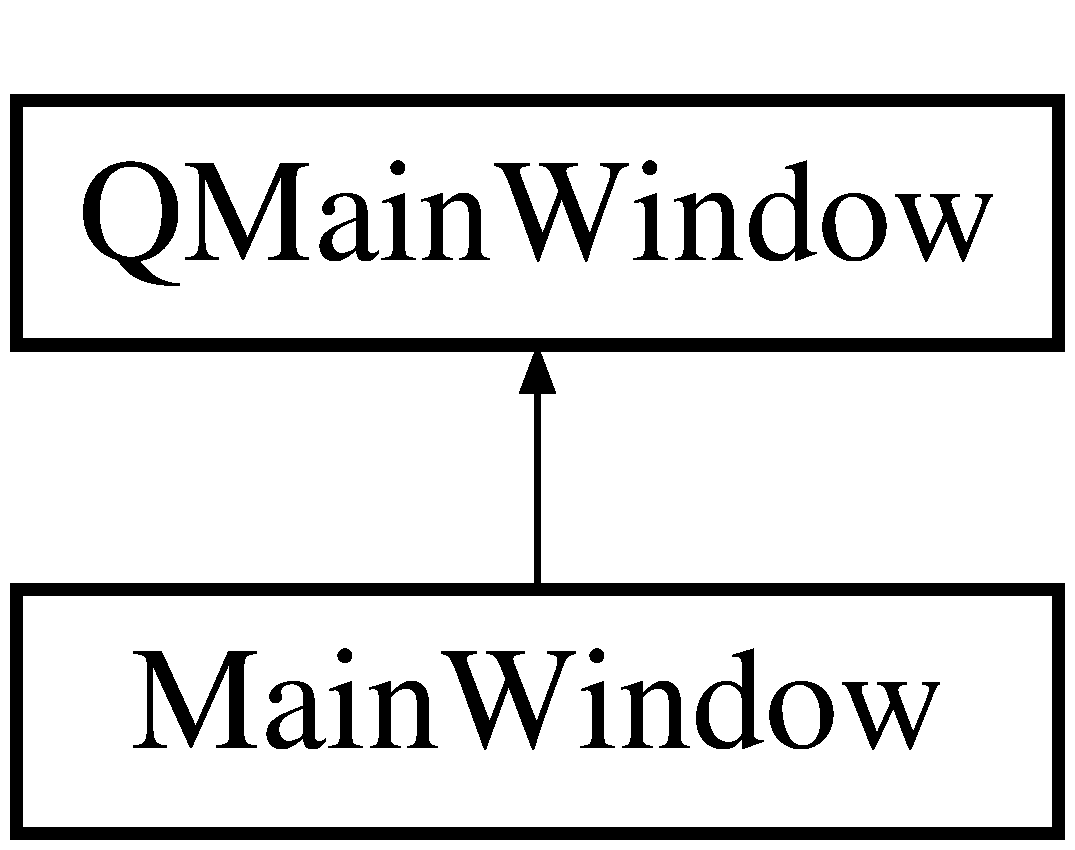
\includegraphics[height=2.000000cm]{class_main_window}
\end{center}
\end{figure}
\subsection*{Public Member Functions}
\begin{DoxyCompactItemize}
\item 
\hypertarget{class_main_window_a8b244be8b7b7db1b08de2a2acb9409db}{{\bfseries Main\+Window} (Q\+Widget $\ast$parent=0)}\label{class_main_window_a8b244be8b7b7db1b08de2a2acb9409db}

\end{DoxyCompactItemize}
\subsection*{Protected Slots}
\begin{DoxyCompactItemize}
\item 
\hypertarget{class_main_window_aa146e796f9a0cfeb05c1ef31a81c6f75}{void {\bfseries on\+\_\+action\+Load\+\_\+\+File\+\_\+triggered} ()}\label{class_main_window_aa146e796f9a0cfeb05c1ef31a81c6f75}

\end{DoxyCompactItemize}
\subsection*{Private Attributes}
\begin{DoxyCompactItemize}
\item 
\hypertarget{class_main_window_a35466a70ed47252a0191168126a352a5}{\hyperlink{class_ui_1_1_main_window}{Ui\+::\+Main\+Window} $\ast$ {\bfseries ui}}\label{class_main_window_a35466a70ed47252a0191168126a352a5}

\item 
\hypertarget{class_main_window_ac7f41407e2c50b7d62e17b7e960ff5d9}{\hyperlink{classglrenderer}{glrenderer} $\ast$ {\bfseries renderer\+\_\+}}\label{class_main_window_ac7f41407e2c50b7d62e17b7e960ff5d9}

\end{DoxyCompactItemize}


The documentation for this class was generated from the following files\+:\begin{DoxyCompactItemize}
\item 
mainwindow.\+h\item 
mainwindow.\+cpp\end{DoxyCompactItemize}

\hypertarget{class_ui_1_1_main_window}{\section{Ui\+:\+:Main\+Window Class Reference}
\label{class_ui_1_1_main_window}\index{Ui\+::\+Main\+Window@{Ui\+::\+Main\+Window}}
}
Inheritance diagram for Ui\+:\+:Main\+Window\+:\begin{figure}[H]
\begin{center}
\leavevmode
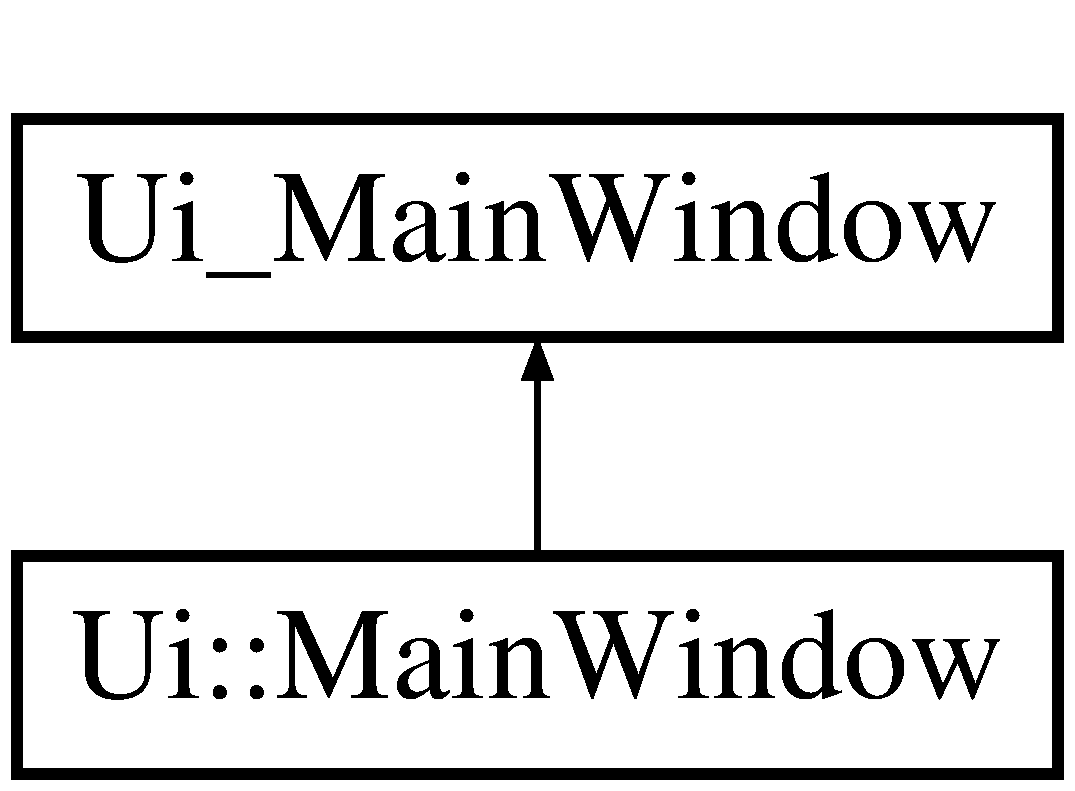
\includegraphics[height=2.000000cm]{class_ui_1_1_main_window}
\end{center}
\end{figure}
\subsection*{Additional Inherited Members}


The documentation for this class was generated from the following file\+:\begin{DoxyCompactItemize}
\item 
ui\+\_\+mainwindow.\+h\end{DoxyCompactItemize}

\hypertarget{classsfe_1_1_sequential_sound_streamer}{\section{sfe\+:\+:Sequential\+Sound\+Streamer Class Reference}
\label{classsfe_1_1_sequential_sound_streamer}\index{sfe\+::\+Sequential\+Sound\+Streamer@{sfe\+::\+Sequential\+Sound\+Streamer}}
}
Inheritance diagram for sfe\+:\+:Sequential\+Sound\+Streamer\+:\begin{figure}[H]
\begin{center}
\leavevmode
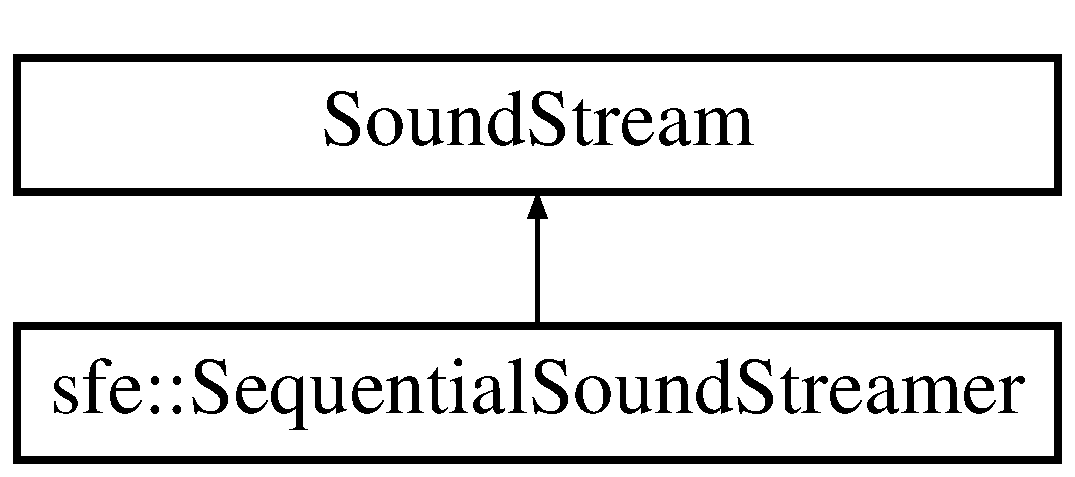
\includegraphics[height=2.000000cm]{classsfe_1_1_sequential_sound_streamer}
\end{center}
\end{figure}
\subsection*{Public Member Functions}
\begin{DoxyCompactItemize}
\item 
\hypertarget{classsfe_1_1_sequential_sound_streamer_a0889a532e125e6229911c87a4411149b}{{\bfseries Sequential\+Sound\+Streamer} (std\+::size\+\_\+t Buffer\+Size)}\label{classsfe_1_1_sequential_sound_streamer_a0889a532e125e6229911c87a4411149b}

\item 
void \hyperlink{classsfe_1_1_sequential_sound_streamer_a650824533bf27a504739798fc4291e69}{load} (const sf\+::\+Sound\+Buffer \&buffer)
\item 
double $\ast$ \hyperlink{classsfe_1_1_sequential_sound_streamer_a54215b061173c1c6b1bebe73a8e79cf0}{get\+F\+F\+T\+Abs} ()
\item 
double $\ast$ \hyperlink{classsfe_1_1_sequential_sound_streamer_a7c94675b37f7f18ae3b535b1c358fb3b}{get\+F\+F\+T\+Phase} ()
\end{DoxyCompactItemize}


\subsection{Member Function Documentation}
\hypertarget{classsfe_1_1_sequential_sound_streamer_a54215b061173c1c6b1bebe73a8e79cf0}{\index{sfe\+::\+Sequential\+Sound\+Streamer@{sfe\+::\+Sequential\+Sound\+Streamer}!get\+F\+F\+T\+Abs@{get\+F\+F\+T\+Abs}}
\index{get\+F\+F\+T\+Abs@{get\+F\+F\+T\+Abs}!sfe\+::\+Sequential\+Sound\+Streamer@{sfe\+::\+Sequential\+Sound\+Streamer}}
\subsubsection[{get\+F\+F\+T\+Abs}]{\setlength{\rightskip}{0pt plus 5cm}double$\ast$ sfe\+::\+Sequential\+Sound\+Streamer\+::get\+F\+F\+T\+Abs (
\begin{DoxyParamCaption}
{}
\end{DoxyParamCaption}
)\hspace{0.3cm}{\ttfamily [inline]}}}\label{classsfe_1_1_sequential_sound_streamer_a54215b061173c1c6b1bebe73a8e79cf0}
returns an array of the magnitude of the transformed data \hypertarget{classsfe_1_1_sequential_sound_streamer_a7c94675b37f7f18ae3b535b1c358fb3b}{\index{sfe\+::\+Sequential\+Sound\+Streamer@{sfe\+::\+Sequential\+Sound\+Streamer}!get\+F\+F\+T\+Phase@{get\+F\+F\+T\+Phase}}
\index{get\+F\+F\+T\+Phase@{get\+F\+F\+T\+Phase}!sfe\+::\+Sequential\+Sound\+Streamer@{sfe\+::\+Sequential\+Sound\+Streamer}}
\subsubsection[{get\+F\+F\+T\+Phase}]{\setlength{\rightskip}{0pt plus 5cm}double$\ast$ sfe\+::\+Sequential\+Sound\+Streamer\+::get\+F\+F\+T\+Phase (
\begin{DoxyParamCaption}
{}
\end{DoxyParamCaption}
)\hspace{0.3cm}{\ttfamily [inline]}}}\label{classsfe_1_1_sequential_sound_streamer_a7c94675b37f7f18ae3b535b1c358fb3b}
returns an array of the phase of the transformed data \hypertarget{classsfe_1_1_sequential_sound_streamer_a650824533bf27a504739798fc4291e69}{\index{sfe\+::\+Sequential\+Sound\+Streamer@{sfe\+::\+Sequential\+Sound\+Streamer}!load@{load}}
\index{load@{load}!sfe\+::\+Sequential\+Sound\+Streamer@{sfe\+::\+Sequential\+Sound\+Streamer}}
\subsubsection[{load}]{\setlength{\rightskip}{0pt plus 5cm}void sfe\+::\+Sequential\+Sound\+Streamer\+::load (
\begin{DoxyParamCaption}
\item[{const sf\+::\+Sound\+Buffer \&}]{buffer}
\end{DoxyParamCaption}
)}}\label{classsfe_1_1_sequential_sound_streamer_a650824533bf27a504739798fc4291e69}
loads data from a sound buffer object 

The documentation for this class was generated from the following files\+:\begin{DoxyCompactItemize}
\item 
Sequential\+Sound\+Streamer.\+h\item 
Sequential\+Sound\+Streamer.\+cpp\end{DoxyCompactItemize}

\hypertarget{class_turing}{\section{Turing Class Reference}
\label{class_turing}\index{Turing@{Turing}}
}
\subsection*{Public Member Functions}
\begin{DoxyCompactItemize}
\item 
\hypertarget{class_turing_a3cad41d7b0d6091a6c884392b1a7ef0e}{{\bfseries Turing} (const int $\ast$acts, const int $\ast$inhibs, const double $\ast$smalls, const int $\ast$w, const int $\ast$syms, const int res\+W, const int res\+H)}\label{class_turing_a3cad41d7b0d6091a6c884392b1a7ef0e}

\item 
\hypertarget{class_turing_a2457d5fc7995a59591277feb4638c065}{void {\bfseries iterate} ()}\label{class_turing_a2457d5fc7995a59591277feb4638c065}

\item 
\hypertarget{class_turing_a07e8488de30f7cfad5a2adb0854877cc}{double $\ast$$\ast$ {\bfseries Get\+Array} ()}\label{class_turing_a07e8488de30f7cfad5a2adb0854877cc}

\item 
\hypertarget{class_turing_a36851de65c0bb0645f055dbcdaf18137}{double {\bfseries Get\+Pixel} (int x, int y)}\label{class_turing_a36851de65c0bb0645f055dbcdaf18137}

\item 
\hypertarget{class_turing_a1ba8305fcdadbddeab2e3da05e15f1be}{void {\bfseries Abs\+Matrix\+Subtract} (double $\ast$$\ast$pos, double $\ast$$\ast$neg, double $\ast$$\ast$dest, int x, int y)}\label{class_turing_a1ba8305fcdadbddeab2e3da05e15f1be}

\end{DoxyCompactItemize}
\subsection*{Static Public Attributes}
\begin{DoxyCompactItemize}
\item 
\hypertarget{class_turing_a7839ff6ada90a2003ec77427a40395e5}{static const int {\bfseries scales} = 5}\label{class_turing_a7839ff6ada90a2003ec77427a40395e5}

\item 
\hypertarget{class_turing_a9122bbf71c58f54167f1ad1b8919b0fb}{static const int {\bfseries varrad} = 2}\label{class_turing_a9122bbf71c58f54167f1ad1b8919b0fb}

\item 
\hypertarget{class_turing_a5c3a33960f324d21686e2fad8dd347fe}{static const int {\bfseries blurnum} = 1}\label{class_turing_a5c3a33960f324d21686e2fad8dd347fe}

\end{DoxyCompactItemize}
\subsection*{Private Member Functions}
\begin{DoxyCompactItemize}
\item 
\hypertarget{class_turing_a3c92f7d32056d6dbe46cc791bf4017f7}{void {\bfseries Init\+Turing} (const int $\ast$acts, const int $\ast$inhibs, const double $\ast$smalls, const int $\ast$w, const int $\ast$syms, const int res\+W, const int res\+H)}\label{class_turing_a3c92f7d32056d6dbe46cc791bf4017f7}

\item 
\hypertarget{class_turing_abdd425de86a79b9ab77ad9be6bc04d93}{void {\bfseries Activator} ()}\label{class_turing_abdd425de86a79b9ab77ad9be6bc04d93}

\item 
\hypertarget{class_turing_a5acb322d6c46047cffdd9c0aca7ce6ac}{void {\bfseries Activator} (int sn)}\label{class_turing_a5acb322d6c46047cffdd9c0aca7ce6ac}

\item 
\hypertarget{class_turing_a1f8cebb9cf68695829a0eca44163f757}{void {\bfseries R\+Activator} ()}\label{class_turing_a1f8cebb9cf68695829a0eca44163f757}

\item 
\hypertarget{class_turing_a35dac5d9f68c690f858a3b060a5b1601}{void {\bfseries R\+Activator} (int sn)}\label{class_turing_a35dac5d9f68c690f858a3b060a5b1601}

\item 
\hypertarget{class_turing_a67b5e46fcb5d46409acb6d07beba9314}{void {\bfseries Inhibitor} ()}\label{class_turing_a67b5e46fcb5d46409acb6d07beba9314}

\item 
\hypertarget{class_turing_a2aacf2a14ec4ce1866320d64d256cd50}{void {\bfseries Inhibitor} (int sn)}\label{class_turing_a2aacf2a14ec4ce1866320d64d256cd50}

\item 
\hypertarget{class_turing_a9103be1d136c471795ef83da5121429e}{void {\bfseries R\+Inhibitor} ()}\label{class_turing_a9103be1d136c471795ef83da5121429e}

\item 
\hypertarget{class_turing_aecf355dd19afccb977f32849e734ec3c}{void {\bfseries R\+Inhibitor} (int sn)}\label{class_turing_aecf355dd19afccb977f32849e734ec3c}

\item 
\hypertarget{class_turing_a5d93b9d90eefec044c19ea86b64905cb}{void {\bfseries Variation} ()}\label{class_turing_a5d93b9d90eefec044c19ea86b64905cb}

\item 
\hypertarget{class_turing_a605968ae274cfe384997af773c560cfc}{void {\bfseries Variation} (int sn)}\label{class_turing_a605968ae274cfe384997af773c560cfc}

\item 
\hypertarget{class_turing_ab35cd4dd6416da85efbc35f4e297d8aa}{void {\bfseries A\+I\+Diff} ()}\label{class_turing_ab35cd4dd6416da85efbc35f4e297d8aa}

\item 
\hypertarget{class_turing_ac72f82d66c0f62615b66684f891e93e9}{void {\bfseries A\+I\+Diff} (int sn)}\label{class_turing_ac72f82d66c0f62615b66684f891e93e9}

\item 
\hypertarget{class_turing_ad947e4f6b08ae9f3b933a91276df344d}{void {\bfseries Update\+Pixels} ()}\label{class_turing_ad947e4f6b08ae9f3b933a91276df344d}

\item 
\hypertarget{class_turing_a86078276c0ebf7144d60c07708d3e421}{void {\bfseries Normalize} ()}\label{class_turing_a86078276c0ebf7144d60c07708d3e421}

\item 
\hypertarget{class_turing_a919317f43dfc9f3727554fac99753db5}{void {\bfseries Set\+A} (int s)}\label{class_turing_a919317f43dfc9f3727554fac99753db5}

\item 
\hypertarget{class_turing_a0e07e6ece3c9438c56bcdcfa21cc155d}{void {\bfseries Set\+I} (int s)}\label{class_turing_a0e07e6ece3c9438c56bcdcfa21cc155d}

\item 
\hypertarget{class_turing_ab7e478862023f611d69351140064ded3}{void {\bfseries Set\+V} (int s)}\label{class_turing_ab7e478862023f611d69351140064ded3}

\item 
\hypertarget{class_turing_aed92fd348c348f10c5d3e7ffce20a054}{void {\bfseries R\+Avg\+M} (double $\ast$$\ast$$\ast$list, int s)}\label{class_turing_aed92fd348c348f10c5d3e7ffce20a054}

\item 
\hypertarget{class_turing_ae4f213fe8dd03a88d3e0646129ceb655}{double {\bfseries Get\+M\+Val} (double $\ast$$\ast$mat, int x, int y)}\label{class_turing_ae4f213fe8dd03a88d3e0646129ceb655}

\item 
\hypertarget{class_turing_a75196d7c35a9773b579e50ec886fffd7}{void {\bfseries Avg\+H} (int r, double $\ast$$\ast$source, double $\ast$$\ast$dest)}\label{class_turing_a75196d7c35a9773b579e50ec886fffd7}

\item 
\hypertarget{class_turing_ad37aeeae70eb8dc32fed1fab814253a9}{void {\bfseries Avg\+V} (int r, double $\ast$$\ast$source, double $\ast$$\ast$dest)}\label{class_turing_ad37aeeae70eb8dc32fed1fab814253a9}

\end{DoxyCompactItemize}
\subsection*{Private Attributes}
\begin{DoxyCompactItemize}
\item 
\hypertarget{class_turing_a834503086ec6e48d169c13a5048a70d6}{int $\ast$ {\bfseries activators}}\label{class_turing_a834503086ec6e48d169c13a5048a70d6}

\item 
\hypertarget{class_turing_a685fb1e8cdd55e677a833232585487bf}{int $\ast$ {\bfseries inhibitors}}\label{class_turing_a685fb1e8cdd55e677a833232585487bf}

\item 
\hypertarget{class_turing_a1582c90c5d4b79422d5fa5613e239d73}{int $\ast$ {\bfseries weights}}\label{class_turing_a1582c90c5d4b79422d5fa5613e239d73}

\item 
\hypertarget{class_turing_a4b6ced77e854b8173eaea69eb5b19f54}{int $\ast$ {\bfseries symmetries}}\label{class_turing_a4b6ced77e854b8173eaea69eb5b19f54}

\item 
\hypertarget{class_turing_a6928df31ab2d0d30078785a686bd7fac}{int {\bfseries res\+Width}}\label{class_turing_a6928df31ab2d0d30078785a686bd7fac}

\item 
\hypertarget{class_turing_adbc9d55e7c3f4ea37eb96e9cd67a5cef}{int {\bfseries res\+Height}}\label{class_turing_adbc9d55e7c3f4ea37eb96e9cd67a5cef}

\item 
\hypertarget{class_turing_aa2d9bd89ddbe7d9f89c24b9a87146a39}{double $\ast$ {\bfseries small\+Amounts}}\label{class_turing_aa2d9bd89ddbe7d9f89c24b9a87146a39}

\item 
\hypertarget{class_turing_a3f8999ed810eb6ae42178121e3c1325c}{double $\ast$$\ast$ {\bfseries pattern}}\label{class_turing_a3f8999ed810eb6ae42178121e3c1325c}

\item 
\hypertarget{class_turing_a32ef6cf7e323f92dc729460943c3ed71}{double $\ast$$\ast$$\ast$ {\bfseries activator\+M}}\label{class_turing_a32ef6cf7e323f92dc729460943c3ed71}

\item 
\hypertarget{class_turing_abd93bc345ff9731a26acaab0fa18a2eb}{double $\ast$$\ast$$\ast$ {\bfseries inhibitor\+M}}\label{class_turing_abd93bc345ff9731a26acaab0fa18a2eb}

\item 
\hypertarget{class_turing_aca854b9315a30392f7d8247d99cc917f}{double $\ast$$\ast$$\ast$ {\bfseries variation\+M}}\label{class_turing_aca854b9315a30392f7d8247d99cc917f}

\item 
\hypertarget{class_turing_af61d6d710eebac2c533263634305ee7c}{double $\ast$$\ast$$\ast$ {\bfseries ai\+Diff\+M}}\label{class_turing_af61d6d710eebac2c533263634305ee7c}

\item 
\hypertarget{class_turing_ac53bb0604b488efdb6438303bd3c481a}{double $\ast$$\ast$ {\bfseries dummy}}\label{class_turing_ac53bb0604b488efdb6438303bd3c481a}

\end{DoxyCompactItemize}
\subsection*{Static Private Attributes}
\begin{DoxyCompactItemize}
\item 
\hypertarget{class_turing_af9ae2c0aa54ca516c5787b6a06c1d173}{static const int {\bfseries a\+Def} \mbox{[}5\mbox{]} = \{100, 64, 16, 4, 1\}}\label{class_turing_af9ae2c0aa54ca516c5787b6a06c1d173}

\item 
\hypertarget{class_turing_a513d70f38cb2adeab2153737c9a06280}{static const int {\bfseries i\+Def} \mbox{[}5\mbox{]} = \{200, 128, 32, 8, 2\}}\label{class_turing_a513d70f38cb2adeab2153737c9a06280}

\item 
\hypertarget{class_turing_a90319b75d195ee274c04ae835c327bc2}{static const int {\bfseries w\+Def} \mbox{[}5\mbox{]} = \{1,1,1,1,1\}}\label{class_turing_a90319b75d195ee274c04ae835c327bc2}

\item 
\hypertarget{class_turing_a6b1d338641fd13916597a1408a38b546}{static const int {\bfseries s\+Def} \mbox{[}5\mbox{]} = \{3,2,2,2,2\}}\label{class_turing_a6b1d338641fd13916597a1408a38b546}

\item 
\hypertarget{class_turing_a5e8d7ff7e6fd3efd794d54c2dee3a20f}{static const double {\bfseries sa\+Def} \mbox{[}5\mbox{]} = \{.\+05, .\+04, .\+03, .\+02, .\+01\}}\label{class_turing_a5e8d7ff7e6fd3efd794d54c2dee3a20f}

\end{DoxyCompactItemize}


The documentation for this class was generated from the following files\+:\begin{DoxyCompactItemize}
\item 
Turing.\+h\item 
Turing.\+cpp\item 
Vars.\+cpp\end{DoxyCompactItemize}

\hypertarget{class_ui___main_window}{\section{Ui\+\_\+\+Main\+Window Class Reference}
\label{class_ui___main_window}\index{Ui\+\_\+\+Main\+Window@{Ui\+\_\+\+Main\+Window}}
}
Inheritance diagram for Ui\+\_\+\+Main\+Window\+:\begin{figure}[H]
\begin{center}
\leavevmode
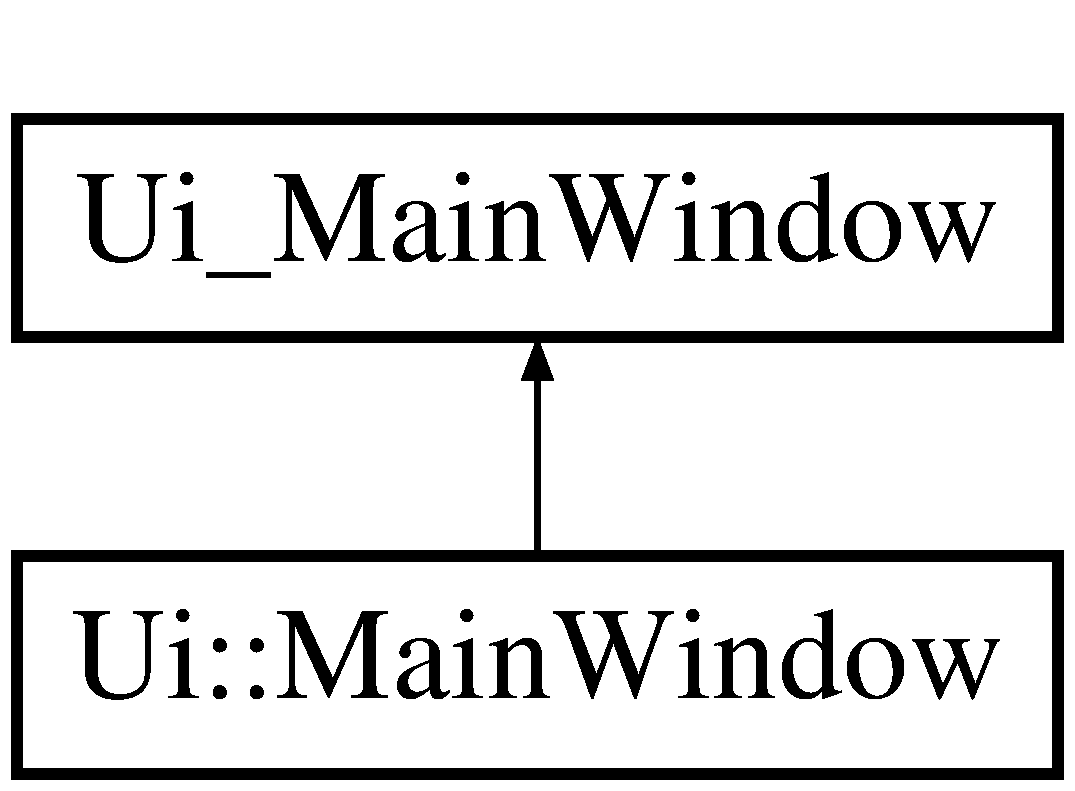
\includegraphics[height=2.000000cm]{class_ui___main_window}
\end{center}
\end{figure}
\subsection*{Public Member Functions}
\begin{DoxyCompactItemize}
\item 
\hypertarget{class_ui___main_window_acf4a0872c4c77d8f43a2ec66ed849b58}{void {\bfseries setup\+Ui} (Q\+Main\+Window $\ast$\hyperlink{class_main_window}{Main\+Window})}\label{class_ui___main_window_acf4a0872c4c77d8f43a2ec66ed849b58}

\item 
\hypertarget{class_ui___main_window_a097dd160c3534a204904cb374412c618}{void {\bfseries retranslate\+Ui} (Q\+Main\+Window $\ast$\hyperlink{class_main_window}{Main\+Window})}\label{class_ui___main_window_a097dd160c3534a204904cb374412c618}

\end{DoxyCompactItemize}
\subsection*{Public Attributes}
\begin{DoxyCompactItemize}
\item 
\hypertarget{class_ui___main_window_a16f32a4d685b6eca5e99051ffdaaa49d}{Q\+Action $\ast$ {\bfseries action\+Load\+\_\+\+File}}\label{class_ui___main_window_a16f32a4d685b6eca5e99051ffdaaa49d}

\item 
\hypertarget{class_ui___main_window_a30075506c2116c3ed4ff25e07ae75f81}{Q\+Widget $\ast$ {\bfseries central\+Widget}}\label{class_ui___main_window_a30075506c2116c3ed4ff25e07ae75f81}

\item 
\hypertarget{class_ui___main_window_a2be1c24ec9adfca18e1dcc951931457f}{Q\+Menu\+Bar $\ast$ {\bfseries menu\+Bar}}\label{class_ui___main_window_a2be1c24ec9adfca18e1dcc951931457f}

\item 
\hypertarget{class_ui___main_window_a7ba84cb4cdd6a12dc83bf4e100bd8d80}{Q\+Menu $\ast$ {\bfseries menu\+File}}\label{class_ui___main_window_a7ba84cb4cdd6a12dc83bf4e100bd8d80}

\item 
\hypertarget{class_ui___main_window_a5172877001c8c7b4e0f6de50421867d1}{Q\+Tool\+Bar $\ast$ {\bfseries main\+Tool\+Bar}}\label{class_ui___main_window_a5172877001c8c7b4e0f6de50421867d1}

\item 
\hypertarget{class_ui___main_window_a50fa481337604bcc8bf68de18ab16ecd}{Q\+Status\+Bar $\ast$ {\bfseries status\+Bar}}\label{class_ui___main_window_a50fa481337604bcc8bf68de18ab16ecd}

\end{DoxyCompactItemize}


The documentation for this class was generated from the following file\+:\begin{DoxyCompactItemize}
\item 
ui\+\_\+mainwindow.\+h\end{DoxyCompactItemize}

%--- End generated contents ---

% Index
\newpage
\phantomsection
\addcontentsline{toc}{chapter}{Index}
\printindex

\end{document}
